\documentclass{article}
\usepackage[a4paper]{geometry}
\usepackage{amsmath}
\usepackage{amsfonts}
\usepackage{amssymb}
\usepackage{graphicx}
\usepackage{float}
\graphicspath{{./images/}}
\begin{document}
\begin{center}
	{\LARGE Exercise 4}\linebreak
	{\large [Avik Banerjee (3374885), Soumyadeep Bhattacharjee (3375428)]}
\end{center}
\textit{Text in italics are notes taken during the tutorial}
\section{Monte Carlo Methods vs Dynamic Programming }
\begin{enumerate}
	\item[a)]
	\begin{itemize}
		\item Monte Carlo methods do not require the knowledge of the environment, particularly the transition probabilities and reward system.
		\item Monte Carlo methods are not biased by the initial conditions of the learning parameters (the initial values assigned to the value functions).
		\item \textit{Less harmed by violations of Markov property, can be used with simulations, model-free, can focus on small subset of state space.}
	\end{itemize}
	\item[b)] Monte Carlo methods are used when it is not possible to have a complete knowledge of all possible state transitions and reward probabilities, such as when trying to teach an agent to play video games where there are millions of possible state and action combinations.
\end{enumerate}
\section{Monte Carlo ES for blackjack}
\begin{enumerate}
	\item[a)] Output plots: \begin{figure}[H]
		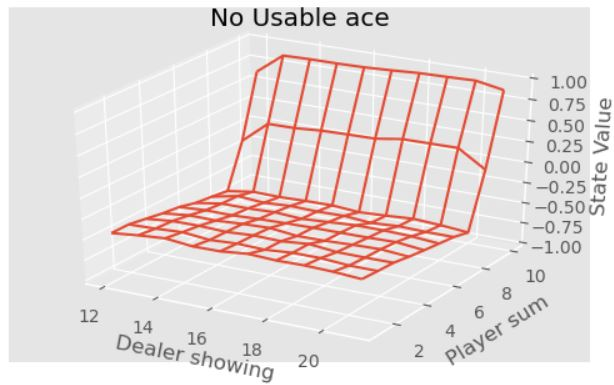
\includegraphics[width=0.5\linewidth]{blackjack1.jpg}
		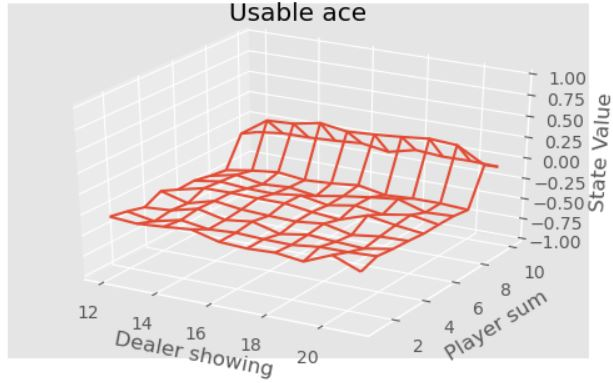
\includegraphics[width=0.5\linewidth]{blackjack2.jpg}
	\end{figure}
\end{enumerate}
\end{document}